\documentclass[11pt,letterpaper]{article}
\usepackage[lmargin=1in,rmargin=1in,tmargin=1in,bmargin=1in]{geometry}
\usepackage{homework}

% -------------------
% Content
% -------------------
\begin{document}
\homework{Solutions --- Caleb McWhorter}

% Problem 1
\problem{10} There are 46~employees at a video game company. The company recently put out an immersive RPG. Of their employees, 14 worked on the story development and 13 worked on the programming, with 3 employees acting as intermediaries between the two groups by working on both. Selecting an employee at random from the company, what is the probability that\dots
        \begin{enumerate}[(a)]
        \item They worked on just the story?
        \item They worked on the game at all?
        \item They did not work on the game at all?
        \item They worked on the story, assuming that they worked on the programming?
        \item A story writer worked on the programming?
        \end{enumerate} \pspace

\sol 
\begin{enumerate}[(a)]
\item 
	\[
	P(\text{just story})= \dfrac{11}{46} \approx 0.2391
	\] 

\item 
	\[
	P(\text{worked on game})= P(\text{story}) + P(\text{prog.}) - P(\text{story and prog.})= \dfrac{14}{46} + \dfrac{13}{46} - \dfrac{3}{46}= \dfrac{24}{46}= \dfrac{12}{23} \approx 0.5217
	\] 

\item 
	\[
	P(\text{not worked on game})= 1 - P(\text{worked on game})= 1 - \dfrac{24}{46}= \dfrac{22}{46}= \dfrac{11}{23} \approx 0.4783
	\] 

\item 
	\[
	P( \text{worked on story} \mid \text{worked on programming})= \dfrac{P(\text{worked on story and prog.})}{P(\text{worked on programming})}= \dfrac{3/46}{13/46}= \dfrac{3}{13} \approx 0.2308
	\] 

\item 
	\[
	P(\text{worked on programming})= \dfrac{13}{46} \approx 0.2826
	\]
\end{enumerate} \vfill

	\[
	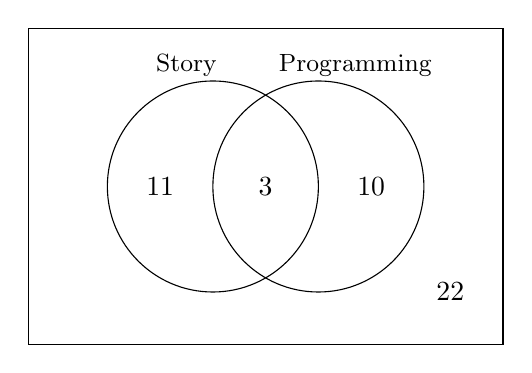
\begin{tikzpicture}[scale=0.67]
	\draw (0,0) rectangle (9,6);
	\draw (3.5,3) circle (2);
	\draw (5.5,3) circle (2);
	
	\node at (3.0,5.3) {\small Story};
	\node at (6.2,5.3) {\small Programming}; 
	
	\node at (2.5,3) {11};
	\node at (4.5,3) {3};
	\node at (6.5,3) {10};
	\node at (8,1) {22};
	\end{tikzpicture}
	\]



\newpage



% Problem 2
\problem{10} A randomized algorithm uses two primary subroutines. The first subroutine is used 20\% of the time and gives a correct computation 59\% of the time, while it crashes 40\% of the time. The second subroutine gives the correct answer 50\% of the time and never crashes.
        \begin{enumerate}[(a)]
        \item Find the probability that the program uses the second subroutine to find the correct answer.
        \item Find the probability that the program gives the correct answer.
        \item Find the probability that the program crashes. 
        \item Find the probability that the program uses the first subroutine, assuming it found the correct answer.
        \item Find the probability that the program used the second subroutine, if the program crashed. 
        \end{enumerate} \pspace

\sol 
\begin{enumerate}[(a)]
\item 
	\[
	P(\text{second sub.})= 0 + 0.40 + 0.40= 0.80
	\] 

\item 
	\[
	P(\text{correct})= 0.0708 + 0.40= 0.4708
	\] 

\item 
	\[
	P(\text{crashes})= 0.08 + 0= 0.08
	\] 

\item 
	\[
	P(\text{first sub.} \mid \text{correct})= \dfrac{P(\text{first sub. and correct})}{P(\text{correct})}= \dfrac{0.0708}{0.4708}= 0.1504
	\] \pspace

\item 
	\[
	P(\text{second sub.} \mid \text{crashed})= \dfrac{P(\text{second sub. and crashed})}{P(\text{crashed})}= \dfrac{0}{0.08}= 0
	\] \pspace
\end{enumerate} \vfill

		\[
		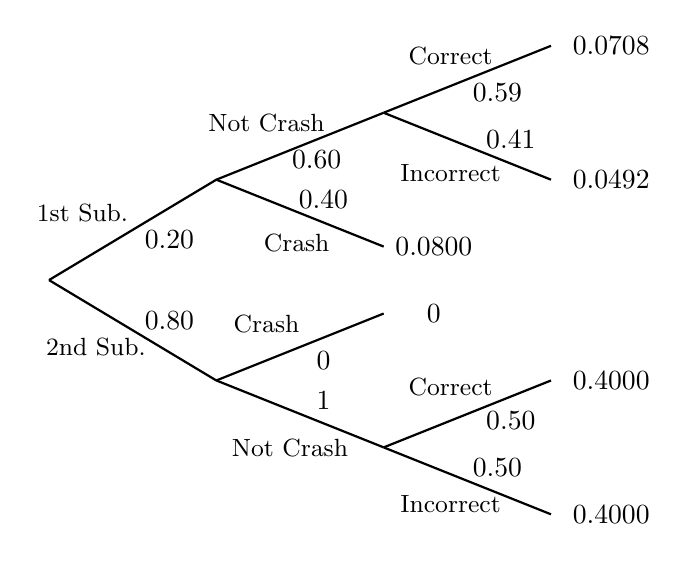
\begin{tikzpicture}[scale= 0.85]
		\def\FirstUpLabel{\small 1st Sub.}
		\def\FirstDownLabel{\small 2nd Sub.}
		\def\SecondUpLabel{\small Not Crash}
		\def\SecondDownLabel{\small Crash}
		\def\Up{$0.20$}
		\def\Down{$0.80$}
		\def\UpUp{$0.60$}
		\def\UpDown{$0.40$}
		\def\DownUp{$0$}
		\def\DownDown{$1$}
		\def\first{$0.0664$}
		\def\second{$0.0800$}
		\def\third{$0$}
		\def\fourth{$0.5612$}
		
		\node at (0.5,1) {\FirstUpLabel};	
		\node at (0.7,-1) {\FirstDownLabel};	
		\node at (1.8,0.6) {\Up};
		\node at (1.8,-0.6) {\Down};
		\draw[thick] (0,0) -- (2.5,1.5);
		\draw[thick] (0,0) -- (2.5,-1.5);
		
		\node at (3.25,2.35) {\SecondUpLabel};
		\node at (3.7,0.55) {\SecondDownLabel};
		\node at (4,1.8) {\UpUp};
		\node at (4.1,1.2) {\UpDown};
		\node at (5.75,0.5) {\second};
		\draw[thick] (2.5,1.5) -- (5,2.5);
		\draw[thick] (2.5,1.5) -- (5,0.5);
		
		\draw[thick] (5,2.5) -- (7.5,3.5);
		\draw[thick] (5,2.5) -- (7.5,1.5);
		\node at (6,3.35) {\small Correct};
		\node at (6.7,2.8) {$0.59$};
		\node at (6,1.6) {\small Incorrect};
		\node at (6.9,2.1) {$0.41$};
		\node at (8.4,3.5) {$0.0708$};
		\node at (8.4,1.5) {$0.0492$};

		\node at (3.25,-0.65) {\small Crash};
		\node at (3.6,-2.5) {\small Not Crash};
		\node at (4.1,-1.2) {\DownUp};
		\node at (4.1,-1.8) {\DownDown};
		\node at (5.75,-0.5) {\third};	
		\draw[thick] (2.5,-1.5) -- (5,-0.5);
		\draw[thick] (2.5,-1.5) -- (5,-2.5);
		
		\draw[thick] (5,-2.5) -- (7.5,-1.5);
		\draw[thick] (5,-2.5) -- (7.5,-3.5);
		\node at (6,-3.35) {\small Incorrect};
		\node at (6.7,-2.8) {$0.50$};
		\node at (6,-1.6) {\small Correct};
		\node at (6.9,-2.1) {$0.50$};
		\node at (8.4,-1.5) {$0.4000$};
		\node at (8.4,-3.5) {$0.4000$};		
		\end{tikzpicture}
		\]



\newpage



% Problem 3
\problem{10} A weighted six-sided die has probabilities (partially) given below: \par
	\begin{table}[!ht]
	\centering 
	\begin{tabular}{|c||c|c|c|c|c|c|} \hline 
	$n$ & $1$ & $2$ & $3$ & $4$ & $5$ & $6$ \\ \hline 
	$P(n)$ & $\dfrac{7}{20}$ & $\dfrac{1}{20}$ & $\dfrac{2}{20}$ & $\mathit{\dfrac{2}{20}}$ & $\dfrac{4}{20}$ & $\dfrac{4\rule{0pt}{2.9ex}}{20\rule[-1.3ex]{0pt}{0pt}}$ \\ \hline
	\end{tabular}
	\end{table} \par
Suppose a game is played using this die where if one rolls a 6, you win \$10, if you roll a 4 or 5 you win nothing, and if you roll a 2 or 3, you lose \$2, and if you roll a 1 you lose \$3. 
        \begin{enumerate}[(a)]
        \item Complete the probability table above.
        \item Find the probability of rolling at least one 6 every 10~rolls. 
        \item Find the expected value. Should one play this game? Explain.
        \item What if one had to pay \$1 to play the game each time? How does this change the answer from (c)? 
        \end{enumerate} \pspace

\sol 
\begin{enumerate}[(a)]
\item We know that\dots
	\[
	\begin{gathered}
	P(X= 1) + P(X= 2) + P(X= 3) + P(X= 4) + P(X= 5) + P(X= 6)= 1 \\
	\dfrac{7}{20} + \dfrac{1}{20} + \dfrac{2}{20} + P(X= 4) + \dfrac{4}{20} + \dfrac{4}{20}= 1 \\
	P(X= 4) + \dfrac{18}{20}= 1 \\
	P(X= 4)= \dfrac{2}{20} \\
	P(X= 4)= \dfrac{1}{10} \approx 0.10
	\end{gathered}
	\]

\item We assume the rolls are independent. We know $P(\text{not } 6)= 1 - P(X= 6)= 1 - \frac{4}{20}= \frac{16}{20}= \frac{4}{5}$. 

But then\dots
	\[
	P(\text{At least one 6})= 1 - P(\text{No 6's in 10 rolls})= 1 - \left( \dfrac{4}{5} \right)^{10}= 1 - \dfrac{1,\!048,\!576}{9,\!765,\!625} \approx 1 - 0.107374= 0.892626
	\]

\item Observe that\dots \par
	\begin{table}[!ht]
	\centering 
	\begin{tabular}{|c||c|c|c|c|c|c|} \hline 
	$n$ & $1$ & $2$ & $3$ & $4$ & $5$ & $6$ \\ \hline 
	$P(n)$ & $\dfrac{7}{20}$ & $\dfrac{1}{20}$ & $\dfrac{2}{20}$ & $\dfrac{2}{20}$ & $\dfrac{4}{20}$ & $\dfrac{4\rule{0pt}{2.9ex}}{20\rule[-1.3ex]{0pt}{0pt}}$ \\ \hline
	Payout & $-\$3$ & $-\$2$ & $-\$2$ & $\$0$ & $\$0$ & $\$10$ \\ \hline 
	\end{tabular}
	\end{table} \par
But then\dots
	\[
	\begin{aligned}
	EX&= \sum x P(x= X) \\
	&= -\$3 \cdot \dfrac{7}{20} + (-\$2) \cdot \dfrac{1}{20} + (-\$2) \cdot \dfrac{2}{20} + \$0 \cdot \dfrac{2}{20} + \$0 \cdot \dfrac{4}{20} + \$10 \cdot \dfrac{4}{20} \\
	&= -\$\dfrac{21}{20} - \$\dfrac{2}{20} - \$\dfrac{4}{20} + \$0 + \$0 + \$\dfrac{40}{20} \\
	&= \$\dfrac{13}{20} \approx \$0.65
	\end{aligned}
	\]
Therefore, after playing `many' games, one expects to have won \$0.65 per game on average; that is, after totaling the net amount won/lost and dividing by the number of games played, one expects an average payout of \$0.65 per game. Because $EX= \$0.65 > 0$, we know that one expects to win money on average. Based on this analysis, one should play the game. \pspace

\item One can recompute the net amount won or lost per game, e.g. if one rolls a 6, then you win \$10 but paid \$1 to play for a net win/loss of $\$10 + (-\$1)= \$9$. This gives the following table: \par 
	\begin{table}[!ht]
	\centering 
	\begin{tabular}{|c||c|c|c|c|c|c|} \hline 
	$n$ & $1$ & $2$ & $3$ & $4$ & $5$ & $6$ \\ \hline 
	$P(n)$ & $\dfrac{7}{20}$ & $\dfrac{1}{20}$ & $\dfrac{2}{20}$ & $\dfrac{2}{20}$ & $\dfrac{4}{20}$ & $\dfrac{4\rule{0pt}{2.9ex}}{20\rule[-1.3ex]{0pt}{0pt}}$ \\ \hline
	Payout & $-\$4$ & $-\$3$ & $-\$3$ & $-\$1$ & $-\$1$ & $\$9$ \\ \hline 
	\end{tabular}
	\end{table} \par
But then the expected value is\dots
	\[
	\begin{aligned}
	EX&= \sum x P(x= X) \\
	&= -\$4 \cdot \dfrac{7}{20} + (-\$3) \cdot \dfrac{1}{20} + (-\$3) \cdot \dfrac{2}{20} + (-\$1) \cdot \dfrac{2}{20} + (-\$1) \cdot \dfrac{4}{20} + \$9 \cdot \dfrac{4}{20} \\
	&= -\$\dfrac{28}{20} - \$\dfrac{3}{20} - \$\dfrac{6}{40} - \$ \dfrac{2}{20} - \$\dfrac{4}{20} + \$\dfrac{36}{20} \\
	&= -\$\dfrac{7}{20} \approx -\$0.35
	\end{aligned}
	\]
Alternatively, recall that if $X, Y$ are discrete random variables and $Y= aX + b$, where $a, b$ are real numbers, then $EY= E(aX + b)= a EX + b$. If $X$ is the payout for the original game, the payout of new game, which we call $Y$, is $Y= X - 1$. But then $EY= E(X - 1)= EX - 1= \$0.65 - \$1= -\$0.35$. \pspace

Using either approach, we have $EX= -\$0.35$. Therefore, after playing `many' games, one expects to have lost \$0.35 per game on average; that is, after totaling the net amount won/lost and dividing by the number of games played, one expects an average loss of \$0.35 per game. Because $EX= -\$0.35 < 0$, we know that one expects to lose money on average. Based on this analysis, one should not play this game. This should make sense. The only difference between the original situation and the current one is now we pay \$1 to play the game. Before, we only won an average amount of \$0.65 per game which is not enough to make up for the \$1 loss before rolling the die. 
\end{enumerate}



\newpage



% Problem 4
\problem{10} A ``$2^2$-face'' in a card game consists of having exactly 2 face cards and exactly 2 two's in one's five card hand. Being dealt five random cards from a standard 52 card deck, find the probability that one receives a ``$2^2$-face.'' \pspace

\sol We know that the probability should be $P(2^2 \text{-face hand})= \tfrac{\text{number } 2^2 \text{-face hands}}{\text{number of 5 card hands}}$. We need only compute this numerator and denominator and we compute these separately. First, we recall a few facts and make a few observations. There are 52~cards in a standard deck consisting of four suits (hearts, spades, diamonds, clubs) that each have the numbers $2, 3, 4, \ldots, 10$, three face cards (jack, queen, king), and an ace. Observe that the order in which the cards are dealt is unimportant---one can always rearrange them in one's hand and it is still the same set of cards. Finally, we cannot have repetition of a \textit{single} card---there is only one card of a specific suit and type in the deck. [Though one can repeat a suit or a type, e.g. hearts or queen.] \pspace

{\itshape Number of five card $2^2$-faces:} One can describe the process of choosing a five card $2^2$-face hand as follows: choose a type of face card (jack, queen, king), choose from those face cards two of them, choose two 2's to be dealt, and then finally choose a fifth card for your hand. Using this breakdown of the process of selecting a $2^2$-face hand, we can use the Generalized Multiplication Principle to compute the number of five card $2^2$-face hands. Observe the order of the card selection does not matter---it is the same hand regardless. Also, observe that there is no repetition (of the exact same card) in the selection. Now there are three types of face cards from which we need to select one type, which can be done in $\binom{3}{1}$ ways. One then needs to select two of the four face cards of the type just selected to include in the hand, which can be done in $\binom{4}{2}$ ways. Then the hand needs to include two of the four possible twos in the deck, which can be done in $\binom{4}{2}$ ways. Finally, one needs to include one other card in the hand. However, this card cannot be a face card or a two. [Otherwise, one would have a full house and not a $2^2$-face hand.] So we choose from the remaining $13 - 4= 9$~card types, which can be done in $\binom{9}{1}$ ways, and then choose one of those four cards to include in the hand, which can be done in $\binom{4}{1}$ ways. [This is the same as choosing one of the cards that is not a face card or a two. There are $52 - 3 \cdot 4 - 1 \cdot 4= 36$ such cards so that the selection can be done in $\binom{36}{1}$ ways.] Therefore, the number of $2^2$-face card hands is\dots
	\[
	\text{Number } 2^2 \text{-face hands}= \underbrace{\binom{3}{1} \binom{4}{2}}_{\text{Choosing Face Cards}} \cdot \underbrace{\binom{4}{2}}_{\text{Choosing 2's}} \cdot \underbrace{\binom{9}{1} \binom{4}{1}}_{\text{Choose Last Card}}= (3 \cdot 6) \cdot 6 \cdot (9 \cdot 4)= 3,\!888
	\] \pspace

{\itshape Number of five card hands:} This is straightforward. From the 52 cards in the deck, we need to choose any five of them to be dealt. The order of the cards does not matter---it is the same hand either way. Moreover, there can be no repetition in the exact cards dealt (the type or suit, but not the \textit{exact} card). Therefore, the number of five card hands is\dots
	\[
	\text{Number five card hands}= \binom{52}{5}= 2,\!598,\!960
	\] \pspace

Therefore, the probability of receiving such a hand is\dots
	\[
	P(2^2 \text{-face hand})= \dfrac{\text{number } 2^2 \text{-face hands}}{\text{number of 5 card hands}}= \dfrac{3,\!888}{2,\!598,\!960}= \dfrac{81}{54,\!145} \approx 0.001495983
	\]
Therefore, there is only a $0.15\%$ chance of receiving such a hand; that is, the odds are 667.457:1. Because five card poker hands are ranked by their odds of occurring,\footnote{Except for a no pair or high card hand which has a probability of 17.4\% chance of occurring, which is lower than a single pair hand. But of course, a no pair/high card hand has `nothing special' about it.} i.e. a one pair hand is lowest at 43.8\% chance and a royal flush is highest at 0.0032\% chance. This would put a $2^2$-face hand as `stronger' than a flush (0.1965\%) but `weaker' than a full house (0.1441\%). 



\newpage



% Problem 5
\problem{10} Find the probability of getting a three of a kind in standard 5~card poker. \pspace

\sol We know that the probability should be $P(\text{three of a kind})= \tfrac{\text{number three kind hands}}{\text{number of 5 card hands}}$. We need only compute this numerator and denominator and we compute these separately. First, we recall a few facts and make a few observations. There are 52~cards in a standard deck consisting of four suits (hearts, spades, diamonds, clubs) that each have the numbers $2, 3, 4, \ldots, 10$, three face cards (jack, queen, king), and an ace. Observe that the order in which the cards are dealt is unimportant---one can always rearrange them in one's hand and it is still the same set of cards. Finally, we cannot have repetition of a \textit{single} card---there is only one card of a specific suit and type in the deck. [Though one can repeat a suit or a type, e.g. hearts or queen.] \pspace 

{\itshape Number of three of a kinds:} One can describe the process of choosing a five card hand with a three of a kind as follows: choose a type of card for the three of a kind, e.g. 2, 5, jack, ace, etc., then choose three of the four possible cards of that type for the hand. We then need to choose two remaining cards for the hand. However, these cannot include the type of card chosen for the three of a kind. [Otherwise, one would have a four of a kind.] These two cards cannot also be of the same type. [Otherwise, one would have a full house.] Therefore, we need to choose two of the remaining types of cards (one not chosen for the three of a kind) without repeating the choice of type. We then choose one of the four cards from each of these two types to include in the hand. Using this breakdown of the process of selecting a three of a kind hand, we can use the Generalized Multiplication Principle to compute the number of five card three of a kind hands. Observe the order of the card selection does not matter---it is the same hand regardless. Also, observe that there is no repetition (of the exact same card) in the selection. From the 13 suits, we need to choose one for the three of a kind, which can be done in $\binom{13}{1}$ ways. We then choose three of the four cards of that type for the three of a kind, which can be done in $\binom{4}{3}$ ways. Then we need to choose two of the remaining $13 - 1= 12$~types of cards, which can be done in $\binom{12}{2}$ ways, and then choose one of the four cards of the first type (which can be done in $\binom{4}{1}$ ways) and choose one of the four cards of the last type (which can be done in $\binom{4}{1}$ ways). Therefore, the number of three of a kind hands is\dots
	\[
	\text{Number three of a kinds}= \underbrace{\binom{13}{1} \cdot \binom{4}{3}}_{\text{Choose Three Pair}} \cdot \underbrace{\binom{12}{1} \binom{4}{1} \binom{4}{1}}_{\text{Choose Last 2 Cards}}= (13 \cdot 4) \cdot (66 \cdot 4 \cdot 4)= 54,\!912	
	\] \pspace

{\itshape Number of five card hands:} This is straightforward. From the 52 cards in the deck, we need to choose any five of them to be dealt. The order of the cards does not matter---it is the same hand either way. Moreover, there can be no repetition in the exact cards dealt (the type or suit, but not the \textit{exact} card). Therefore, the number of five card hands is\dots
	\[
	\text{Number five card hands}= \binom{52}{5}= 2,\!598,\!960
	\] 

Therefore, we have\dots
	\[
	P(\text{three of a kind})= \dfrac{\text{number three kind hands}}{\text{number of 5 card hands}}= \dfrac{54,\!912}{2,\!598,\!960}= \dfrac{88}{4165} \approx 0.021128451
	\]
Therefore, the probability of receiving a three of a kind is approximately 2.113\%. 


\end{document}